\chapter{Introduction}

There is an increasing awareness of the potential benefits of intelligent energy control of the balance between the distributed energy resources and the demand requirements. Intelligent energy control leads to efficient planning, more satisfied consumers and can even help National Electricity Markets in saving considerable operating and maintenance cost according to \cite{NarjesFallah2018}. Having accurate forecasting models is one of the key conditions to in practise realize intelligent energy control. When electricity consumption forecasting is improved, energy producers can build a better trust with its customers by sending reliable bills. Furthermore, can the electricity producer better estimate the energy demand of the whole customer population. The optimization of the energy production planning is possible, which will lead to cheaper electricity production and increased profit margins. More substantiated decisions can be taken with regard to investments and there will be less need of the more flexible, but more expensive electricity installations e.g. diesel engines, to catch the deficiencies in electricity production.\\

\begin{figure}[h!]
	\centering
	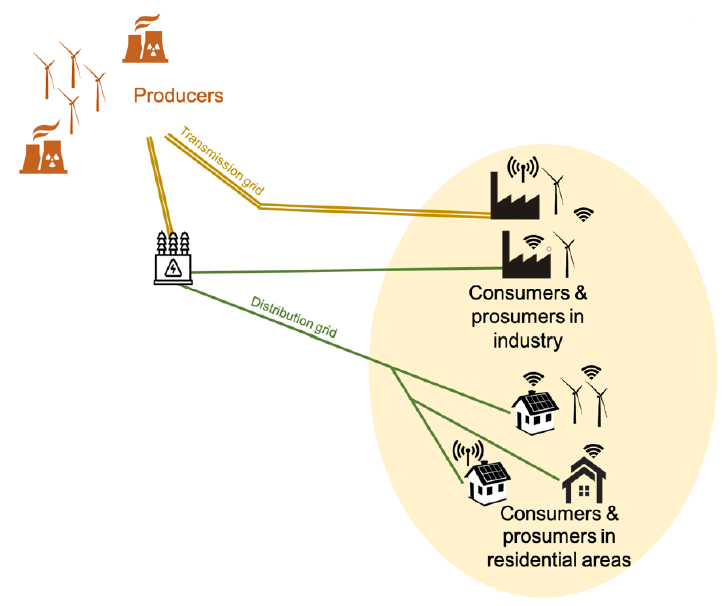
\includegraphics[width=0.8\textwidth]{SmartGrid.png}
	\caption{Electricity grid (Source: KU Leuven thesis proposal).}
	\label{fig:power_image}
\end{figure}

With the invention of the smart meter in 1974 by \textbf{Paraskevakos}, it became possible to communicate the electricity consumption with more clarity to the electricity consumer and producer. Electricity consumption is nearly recorded real time and a smart meter allows for two-way communication between the smart meter and the supplier. As explained in \cite{Depuru2011}: ``By introducing smart meters as a new
component of their smart grid system, an avalanche of immensely useful energy usage information
became available to the energy markets.'' From the availability of more detailed datasets comes the explosion of research in the area of electrical forecasting techniques and the applicability of more complex models. To tackle the electrical consumption forecasting problem also machine learning techniques as neural networks are applied. These models allow for learning very non-linear relations between the inputs and output. Learning is done by updating the model every time such that the observations in the training set are better explained.\\

In \cite{NarjesFallah2018} different forecasting horizons are discussed with their practical application. This is summarized in Table \ref{tab:prediciontypes}.

\begin{table}[h!]
	\centering
	\begin{tabular}{@{}lp{3cm}p{3cm}p{4.5cm}@{}} \toprule
		\textbf{Acronym}	& \textbf{Prediction type} & \textbf{Time span} & \textbf{Application}\\\midrule
		VSTLF	& Very short Term Load Forecasting	& One minute to an hour	& Operational and maintenance
		scheduling and Demand side management
		(decision making for load
		control and voltage reduction)\\\hline		
		STLF	&	Short Term Load Forecasting 	& 	Daily or weekly		& Distribution and transmission
		planning and Demand side management
		(decision making for load
		control and voltage reduction)\\\hline	
		MTLF	&	Medium Term Load Forecasting	& A month to a few years	& Finance or power supply planning\\\hline
		LTLF	&	Long Term Load Forecasting	&	A year to a few decades	&	Finance or power supply planning\\\bottomrule
	\end{tabular}
	\caption{Prediction types that are mentioned in \cite{NarjesFallah2018}.}
	\label{tab:prediciontypes}
\end{table}

The forecast horizon is chosen in consultation with the uncertainty that is contained in the signal. If the signal doesn't show clear patterns, forecasting will be more difficult which means that the forecasting horizon will be shorter. In this thesis the forecasting horizon falls in the category of ``VSTLF'' and ``STLF'' because the consumption is predicted with a frequency of 30 minutes for a duration of 24 hours. The practical application of the developed models in this thesis have indeed as goal to monitor the demand side of the low voltage distribution grid.
Typical inputs that are used in literature for electrical load forecasting are past values of the load, weather information, calendar information and error-correction terms according to \cite{loadforecastingmoor}. Often used inputs for electrical load forecasting are summarized here.

\begin{itemize}
	\item Historical data e.g. \cite{Kong2019}
	\item Weather information
	\begin{itemize}
		\item Temperature e.g. \cite{Kong2019}
		\item Cloudiness e.g. \cite{Contaxi2006}
		\item Humidity e.g. \cite{Contaxi2006}
		\item Wind e.g. \cite{Charytoniuk1997}
	\end{itemize}
	\item Day of the week e.g. \cite{Kong2019}
	\item Time of the day e.g. \cite{Kong2019}
	\item Holiday e.g. \cite{Kong2019}
	\item Anthropological data : Social aspects of the community, general behaviour of house
	occupants e.g. \cite{Javed2012}
	\item Structural data : physical properties of the house e.g. \cite{Javed2012}
\end{itemize}

These inputs are often first normalized before training for which min-max normalization and one hot encoding can be used.

\section{Importance of topic}
This research on short term load forecasting is done in the context of an increased adoption of solar panels and electric cars by the big public. Every year 40000 new solar panel installations take place in Flanders as explained in \cite{Lemmens2019}. Fluvius, which is a Belgian distribution grid operator, has carried out together with Deloitte in 2019 an unique stress test on the low voltage distribution grid to analyse how the current grid will react on the burden of an increased amount of charging points and solar panels. It was found that on the short term, which means up to 2025, the grid will be able to cope with the estimated increase of the burden on the low voltage grid. However, now is the time of anticipation and to strengthen the weak spots in the network. To carry out the maintenance work, detailed forecasting of the load signals of only a small amount of households is needed. Detailed forecasts of individual households is now possible because of the use of smart meters. If detailed predictions are achieved for individual households, expenses are saved because customized updates of the network can be done. With forecasts on the household level, a plan can be made where certain parts of the grid have to be replaced and by how much. Replacing everything is avoided. Individual household predictions can be used as part of an electrical congestion prediction, which means predicting when the low voltage grid can't handle the demand anymore. Especially, predicting the peaks in the household loads is in that case important. If an accurate congestion prediction can be made, reliability of the network can be increased and the risk for blackouts and brownouts is decreased.\\

\section{Problem formulation and link with previous studies}
As discussed in \cite{Shi2018}, the complexity of the household forecasting lies in the significant uncertainty and volatility of the load signal. Uncertainty comprises the aperiodic part influenced by external factors e.g. customer behaviour and weather. Forecasting at the household level makes the load signal to be directly influenced on the decisions made by the residents. In order to attain good results it is found in literature that often aggregated load signals are considered as done in \cite{loadforecastingmoor}. This makes that the uncertainty will be cancelled out and the load signal will show more clear patterns which are easier to model. However, this doesn't allow for individual household forecasting. If there are papers that discuss load forecasting of an individual household, they often use a lot of information about the household situation and submeters to measure the consumption of different appliances or parts of the house as done in \cite{Kim2019}. This will in practise not be scalable due to privacy concerns. This thesis investigates state of the art time series forecasting techniques based on LSTM neural networks that have as goal to directly learn the uncertainties on the load signals, given only limited information.\\

Data from Fluvius of load signals of Belgian households was not available during this thesis. Therefore, data is used from the \href{https://ieee-dataport.org/competitions/ieee-cis-technical-challenge-energy-prediction-smart-meter-data}{IEEE-CIS technical challenge on energy prediction from smart data}. This dataset consists out of 3248 smart meter time series form the UK during the year 2017. In Chapter \ref{cha:State of the art short-term residential load forecasting techniques} a literature study is done about the state of the art short-term residential load forecasting techniques. 


\section{Thesis objective and structure}
The goal of this thesis is to implement short-term load forecasting for individual households when using only a limited amount of information. Concrete, this means that first the question of how much electricity a certain household will consume tomorrow, is tried to be answered. For this, it is looked at LSTM neural networks to predict a load signal of 24 hours ahead with time steps of 30 minutes. Information used about the household only consists of past load values, calendar information and the daily average temperature of tomorrow. These inputs can easily be obtained in practise without intruding the privacy of the residents. The three households used, originate form the IEEE-CIS technical challenge dataset. Because of the use of real-life data, there is a direct link with reality, but the developing of the models is also more challenging due to the anomalies and missing values that are present in the data. The second part of the thesis objective is to evaluate the forecasting performance of the different developed models. To be able to develop the models I had to get familiar with: scikit-learn, Jupyter Notebook, Tensorflow, Keras, Pandas, Anaconda and Microsoft Azure. Therefore, completing this thesis was an educational experience that improved my software skills.\\ 

The structure of the thesis is as follows. First, an exploratory data analysis conducted on the dataset from the IEEE-CIS technical challenge is presented in Chapter \ref{cha:Data analysis}. In this chapter the goal is to look for general characteristics in the data. Only the 261 load series with a full year of smart meter measurements are assessed. In section \ref{s:Preprocessing} it is looked at the missing values, zero days, normalization and shifts in the rolling mean load. Next, in Section \ref{s:Data Analysis} all the 261 load series with a full year of smart meter measurements are aggregated to identify general characteristics of the data. In this section seasonality, comparing electrical consumption between weekdays and weekends, impact of an holiday on the load signal, the influence of the temperature and the identification of the influence of properties of the household e.g. dwelling type is looked at. This last part was possible due to the availability of extra information through a voluntary questionnaire.\\
In Chapter \ref{cha:State of the art short-term residential load forecasting techniques} the literature study that is done is explained. First, an introduction is given about neural networks and the difficulties and solutions are discussed in Section \ref{s:Problems}. Next follows the explanation of the more advanced LSTM and GRU neural networks in respectively Section \ref{s:LSTM} and \ref{s:GRU}, which are specialized in handling time series data. Finally, the introduction to neural networks ends with the explanation of what was found in literature concerning the performance of different parameter settings and different LSTM neural networks in Section \ref{s:Performance results between different models}. The second part of the literature study covers the use of LSTM models for short-term residential electrical load forecasting in Section \ref{s:Short-Term residential electrical load forecasting}.\\
In Chapter \ref{cha:Forecasting the daily electricity consumption} three households are selected from the IEEE-CIS technical challenge dataset with the least amount of missing values. The corresponding load signals are used for individual household forecasting. In section \ref{s:Preprocessing_cha4} the raw data is introduced and preprocessing steps done are explained. Next, Section \ref{s:Error metrics} discusses the error metrics that are used to evaluate the prediction performance of the models. Section \ref{s:Microsoft Azure cloud} clarifies how Microsoft Azure is used for cloud computing. Section \ref{s:Baseline models} describes the development of baseline models that serve as a benchmark for the more complex Deep LSTM models shown in Section \ref{s:Deep LSTM models}. Section \ref{s:Developed models} and \ref{s:Parameter search} discusses respectively the developed models and the parameter search. Chapter \ref{cha:Model evaluation} shows the results of the developed LSTM models on the test set with respect to two selected baseline models. Finally, the conclusion of the thesis follows in Chapter \ref{cha:conclusion}.





%%% Local Variables: 
%%% mode: latex
%%% TeX-master: "thesis"
%%% End: 
